
\chapter{INTRODUÇÃO}


O sucesso de uma cadeia de suprimentos pela perspectiva da indústria pode ser calculado a partir dos KPIs (\textit{Key Performance Indicator}) desenvolvidos pela mesma. Porém diferente de muitos outros setores, a industria tem poucos KPIs relacionados à cadeia de suprimentos e mesmo os existentes não são difundidos dentre as mesmas, e pouco se sabe sobre processos e criação de KPIs diretamente relacionados à cadeia de suprimentos \cite{chae2009developing}.

Um dos problemas da industria alimentícia, principalmente a de produtos perecíveis, é como calcular a quantidade de cada SKU (\textit{Stock Keeping Unit}) a ser fabricada nos próximos meses; já que o estoque, nesses casos,  além de capital parado, corre o risco de não chegar às prateleiras do comércio, e quando chega, tem seu tempo de prateleira significantemente reduzido. Em contrapartida, fabricar produtos a baixo da demanda do mercado leva a perda de receita \cite{aburto2007improved}.

Grande parte das industrias produtoras de alimento em países em desenvolvimento ainda utilizam sistemas arcaicos em conjunto com predições intuitivas para projetar sua produção. Quando a demanda é sazonal, é ainda mais dificil de calcular a produção de algum SKU, causando as perdas mencionadas anteriormente \cite{yenradee2001demand}. Para resolver os problemas supracitados, este trabalho visa avaliar as técnicas atuais de previsão de demanda visando a perspectiva da industria.

\section{Objetivos}
Este trabalho tem como objetivo avaliar as técnicas atuais de previsão de demanda em uma cadeia de suprimentos com foco na visão da industria produtora, visando auxiliar a industria a gerenciar sua produção futura baseada nas suas vendas.
Os objetivos específicos desse trabalho incluem:
\begin{itemize}
\item{Identificar as técnicas de previsão de demanda recomendads pelo meio acadêmico e utilizadas na industria}
\item{Identificar os dados utilizados para fazer a previsão de demanda.}
\end{itemize}

\section{Organização do Trabalho}
Este trabalho será organizado como descrito a seguir:
\begin{itemize}
\item{O Capítulo \ref{theory} descreve os conceitos de Cadeia de Suprimentos, Calculo de Previsão e Aprendizado de Máquina}
\item{O capitulo \ref{revision} apresenta o mapeamento sistemático da literatura visando obter os trabalhos relacionados a este}
\end{itemize}

\chapter{Fundamentação Teórica}\label{theory}

Neste capítulo, serão explorados os conceitos utilizados nesse trabalho, dentre eles conceitos específicos sobre uma cadeia de suprimentos  e sobre aprendizado de máquina, em específico análise de séries temporais.

\section{Cadeia de Suprimentos}

\section{Aprendizado de Maquina}

\subsection{Séries Temporais}


\chapter{Revisão da Literatura} \label{revision}



\section{\esp Inserções de ilustrações}

% Figura
\begin{figure}[ht]
	\centering	
	\caption[\hspace{0.1cm}Grade Computacional.]{Uma Grade Computacional como fonte transparente}
	\vspace{-0.4cm}
	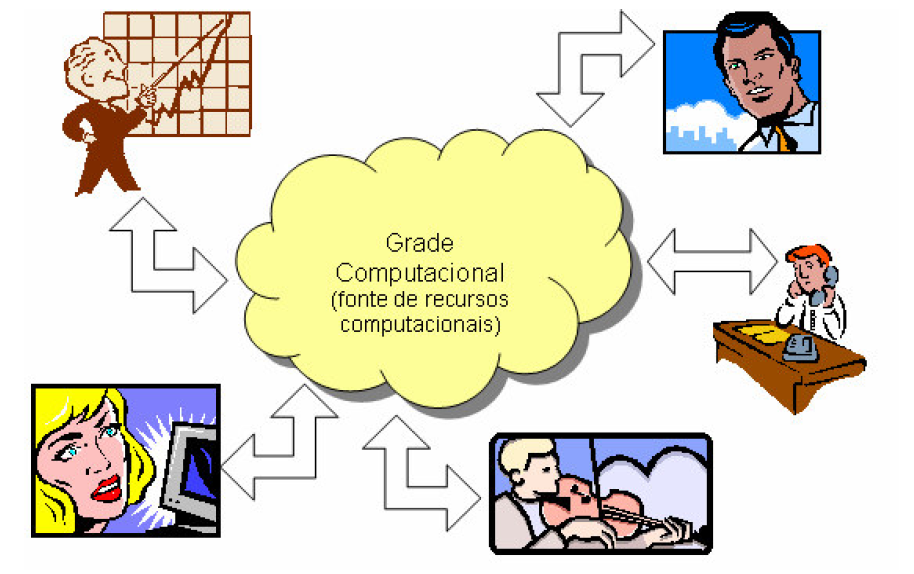
\includegraphics[width=0.6\textwidth]{figuras/grade-comp.png}
	\\\textbf{\footnotesize Fonte: \citeCitacao{cap-livro} }
	\label{fig:figura1}
\end{figure}
\vspace{-0.5cm}

\section{\esp Inserção de tela de software}

% Figura
\begin{figure}[!ht]
	\centering	
	\caption[\hspace{0.1cm}Exemplo de tela de software.]{Exemplo de tela de software}
	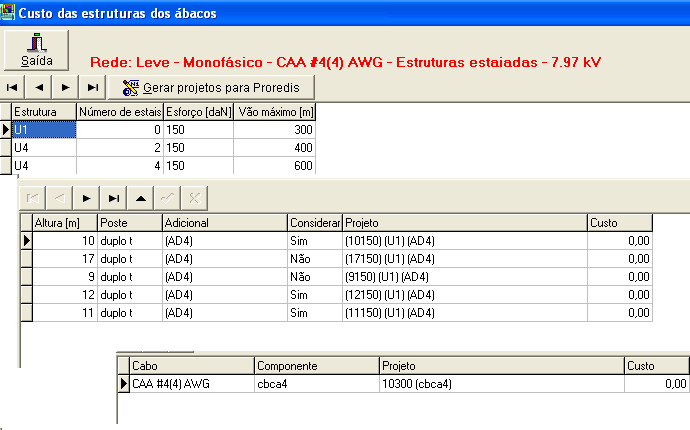
\includegraphics[width=.8\textwidth]{figuras/tela1.png}
	\\\textbf{\footnotesize Fonte: \citeCitacao{tela1}}
	\label{fig:tela1}
\end{figure}

\section{\esp Inserção de gráficos e mapas}

\begin{grafico}
	\centering	
	\graficos{Exemplo de um gráfico}
	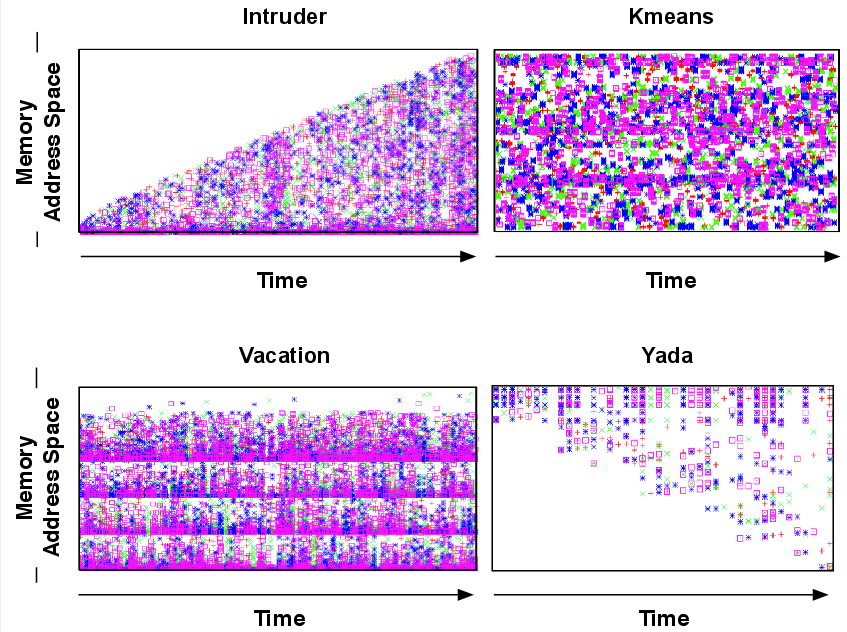
\includegraphics[width=0.7\textwidth]{figuras/access.png}
	\\\textbf{\footnotesize Fonte: \citeCitacao{tese}}
	\label{gra:grafico1}
\end{grafico}


 \section{\esp Tabelas}

% Tabela
\begin{table}[htb]
	\centering
	\caption{\hspace{0.1cm} Exemplo de uma tabela}
	\vspace{-0.3cm} % espaço entre titulo e tabela
	\label{tab:tabela1}
	% Conteúdo da tabela
	\begin{tabular}{l|c|c}
  \hline
    \textbf{Imagem}	& \textbf{transferência} & \textbf{tempo} \\
    \hline
     estação 1	& 7,72 MB/s &  1:22:18 \\
     estação 2	& 7,72 MB/s &  1:22:17 \\
     estação 3	& 7,59 MB/s & 1:24:25 \\
     estação 4  & 7,53 MB/s & 1:43:27 \\
     estação 5	& 6,14 MB/s  &  1:24:41 \\
     estação 6  &  7,50 MB/s & 1:23:53 \\
     estação 7  & 7,58 MB/s  &  1:24:02 \\
     estação 8  & 7,8 MB/s  &  1:29:06 \\
     estação 9  & 7,9 MB/s  &  1:30:05 \\
     estação 10 & 8,0 MB/s  &  1:32:03 \\
     \hline
 \end{tabular}
	\small
	{\footnotesize\\ \textbf{Fonte: \citeCitacao{monog-fabio}}}
\end{table}


\section{\esp Inserção de algoritmos}

\begin{algoritmo}
	\footnotesize
	\algoritmos{Algoritmo genético simples}
	\label{alg:ag}
    \begin{algorithmic}[1]
    		\State Inicialize as probabilidades de cruzamento e mutação, e tamanho da população.
		\State Gere população inicial
		\While{critério convergência não alcançado}
			\State Avalie os indivíduos da população
			\State Execute a seleção
			\State Execute cruzamento
			\State Execute mutação
		\EndWhile{}
  	\end{algorithmic}
	\textbf{\small{Fonte: Adaptado de~\citeCitacao{mestrado}.}}
\end{algoritmo}

\chapter{ CITAÇÕES}


Referências deverão ser adicionadas no arquivo \textit{bibliografia.bib}. Cada referência deverá ser adicionada conforme o padrão de normalização da PUC, 
o qual poderá ser consultado na página da biblioteca da PUC Minas \cite{manualpuc}. Todas as publicações citadas no texto deverão ter correspondente nas referências, 
e as indicações de autoria da citação e do ano deverão ser idênticas aos dados expostos.


\section{\esp Citação livre ou indireta}

Quando se reproduzir ideias, sem transcrever as palavras do autor, a indicação da página é opcional. Exemplos desse tipo de citação:
\begin{enumerate} 
 \item [a)] Citação com um autor \cite{knuth}. 
 \item [b)] Citação de artigos em revistas com dois autores \cite{artigo01}.
  \item [c)] Trabalho em congresso com três autores \cite{dovzan:01}.
 \item [d)] Trabalhos com mais de três autores \cite{cap-livro}.
 \item [e)] Dois autores em duas obras distintas \cite{knuth,groupp}.
 \item [d)] Trabalhos distintos com vários autores \cite{congresso,cap-livro}.
 
\end{enumerate}

\section{\esp Citação direta ou textual}

Transcrição literal de textos de outros autores. Nesse caso, deverão ser especificadas as páginas consultadas. 
Se desejar, poderão ser grafadas em itálico para melhor visualização.

\subsection{\esp Textual Curtas}

Quando curtas (até 3 linhas) serão inseridas na sequência normal do texto, entre aspas com as mesma formatação.

\subsection{\esp Textual Longas}

Citações longas (mais de 3 linhas) deverão constituir um parágrafo independente, recuado a 4 cm da margem esquerda, 
com letra tamanho 10 e digitado em espaço simples, sem aspas.
\begin{citacaodireta}
Hegel chama trabalho à forma específica da satisfação das necessidades, que
distingue da natureza o espírito existente. Assim como a linguagem infringe
a imposição da intuição e ordena o caos das múltiplas sensações em coisas
identificáveis, assim o trabalho infringe a imposição do \hspace{0.1cm}desejo \hspace{0.1cm}imediato \hspace{0.1cm}e
suspende, por assim dizer, o processo de satisfação das necessidades.
\cite[25]{habermas}.
\end{citacaodireta}


% Artigo \cite{whatershed:01}

\subsection{\esp Textual de outros idiomas (Tradução)}

\begin{citacaodireta} 
Um \textit{cluster} é um computador paralelo construído de componentes e processos de \textit{software} (tal como sistema de \textit{software}). 
Um \textit{cluster} é formado de nós, cada um contendo um ou mais processadores, memória que é compartilhada por todos os processadores do nodo 
(somente eles), e dispositivos periféricos adicionais (tais como discos), conectados pela rede e que permitem tráfego de dados entre os nós...
\cite[p. 10, tradução nossa]{groupp}\footnote {  … a cluster is a parallel computer that is constructed of commodity  componets and runs 
(as its system software) commodity software. A cluster is made of nodes, each conteining one or more processors, memory that is  shared 
by all of the processors in (and only on) the node, and addtional peripheral devices (surch as disks),
 connected by network that allows data to move between the nodes}.
\end{citacaodireta}
 
\section{\esp Exemplos de citações} 

Alguns exemplos de citações mais utilizadas e/ou que geram algumas dúvidas. É válido observar que não citaremos
todas as possibilidades de citações da norma da PUC Minas, sendo assim é de extrema relevância que se consulte 
o documento no site da Biblioteca da PUC Minas para maiores esclarecimentos acerca de citações \cite{manualpuc}.

\subsection{\esp Citação de monografia, dissertação e tese}

Exemplo de citação de monografia de curso de graduação ou especialização pode ser vista em \citeonline{monog-fabio}.
Exemplo de dissertação de mestrado é referida como \citeonline{mestrado}.

Para o caso de doutorado é citado da seguinte forma, Góes (\citeyear{tese}). Nesse exemplo é válido observar a forma
como está escrito no documento \LaTeX, pois citações que compreendem no texto o nome do autor como sua parte, necessitam 
do parâmetro \verb$\citeonline{}$. 

\subsection{\esp Livros e partes de livros}

Exemplo de capítulo de livro fica conforme este exemplo \cite{cap-livro}.

Para livros citados no corpo do texto e com duas citações juntas, ver os exemplos \citeonline{knuth,groupp}.
Caso essa citação não fizesse parte do texto será referencia dessa forma \cite{knuth,groupp}.

Citações institucionais ou documentos técnicos de alguma entidade devem ser citados desta forma \cite{pmbok}.

\subsection{\esp Tela de software}

Para  citar a tela de um \textit{software} faça da seguinte forma, \citeonline{tela1}.

\subsection{\esp Citações da Biblia Sagrada}

A Bíblia está dividida em duas grandes partes: O Antigo Testamento e o Novo Testamento, divididos em livros, capítulos e versículos. 
Portanto, a citação de partes da Bíblia deve apresentar o título do livro de forma abreviada ou por extenso, o número do capítulo e o número do versículo.


\begin{citacaodireta}
Moisés estendeu a mão sobre o mar. Com um forte \hspace{-0.1cm} vento \hspace{0.1cm} leste a \hspace{0.1cm}sobrar a
noite toda, o Senhor repeliu o mar e o pôs a seco. As águas se fenderam e
os filhos de Israel entraram no meio do mar a pé enxuto, enquanto as águas
formavam uma muralha à direita e à esquerda deles (\citeauthor{biblia} 14,21).
\end{citacaodireta}

\chapter{ CONCLUSÃO}

Discussão dos resultados obtidos na pesquisa. É onde se colocam as observações do autor. 
Poderá também apresentar sugestões de novas linhas de estudo.

A conclusão deve estar de acordo com os objetivos do trabalho.

A conclusão não deve apresentar citações ou interpretações de outros autores.

 \section{\esp Trabalhos futuros}
% 
 Sugestões de estudos posteriores são ser adicionados subseção deste capítulo de conclusão.
